\section{System Architecture}
\label{sec:architecture}

\begin{figure*}[ht]
\centering
\vspace{0pt}
\begin{minipage}[c]{.4\paperwidth}
\begin{center}
	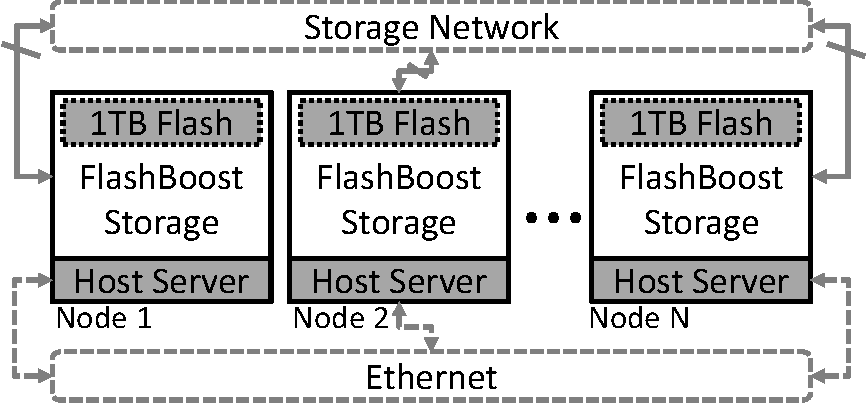
\includegraphics[width=\textwidth]{figures/architecture_small-crop.pdf}
	\caption{FlashBoost Overall Architecture}
	\label{fig:architecture}
\end{center}
\end{minipage}\hfill
\vspace{0pt}
\begin{minipage}[c]{.4\paperwidth}
\begin{center}
	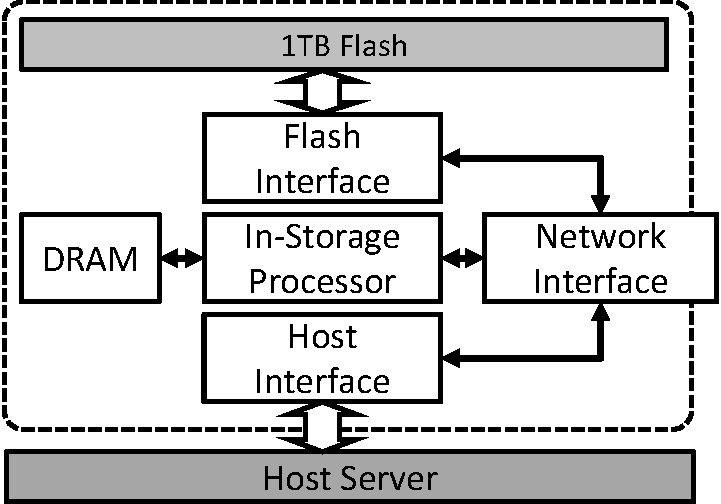
\includegraphics[width=0.7\textwidth]{figures/architecture_node-crop.pdf}
	\caption{FlashBoost Node Architecture}
	\label{fig:architecture_node}
\end{center}
\end{minipage}
\end{figure*}


The FlashBoost architecture is a homogeneous cluster of host servers coupled
with a FlashBoost storage device. Each FlashBoost storage device is plugged into
the host server via a PCIe link, and it consists of flash storage, an in-storage
processing engine, 8 high-speed network interfaces and on-board DRAM. The host
servers are networked together using Ethernet or other general-purpose
networking fabric. The host server can access the FlashBoost storage device via
a host interface implemented over PCIe. It can either directly communicate with
the flash interface, to treat is as a raw storage device, or with the in-store
processor to perform computation on the data.

The in-store processing engine has access to four major services: The flash
interface, network interface, host interface and the on-storage DRAM buffer.
Figure~\ref{fig:architecture_node} shows the four services available to the
in-storage processor. In the following sections we describe the flash interface,
network interface and host interface in order. We omit the DRAM buffer because
its design is very generic.

\subsection{Flash Interface}

Flash devices or SSDs achieve high bandwidth by grouping multiple flash chips
into several channels, all of which can operate in parallel. Because NAND flash
has limited program/erase cycles and frequent errors, complex flash management
algorithms are required to guarantee reliability. These include wear leveling,
garbage collection, bit error correction and bad block management. These
functions are typically handled by multiple ARM-based cores in the SSD
controller. The host side interface of an SSD is typically SATA or PCIe, using
AHCI or NVMe protocols to communicate with host. SSDs are viewed
as a typical block device to the host operating system, and its internal
architecture and management algorithms are completely hidden. 

However, this additional layer of management has shown to be duplicated with
file system functionalities and adds significant latency~\cite{redo}.
Furthermore, in a distributed storage environment, such as FlashBoost,
independent flash devices do not have a holistic view of the system and thus
cannot efficiently manage flash. Finally, in-store processors that we have
introduced in FlashBoost would also incur performance penalties if passing
through this extra layer. 

Thus in FlashBoost, we chose to shift flash management
away from the device and into file system/block device driver (discussed in
Section~\ref{sec:software}). Our flash controller exposes a low-level, thin,
fast and bit-error corrected hardware interface to raw NAND flash chips, buses,
blocks and pages. This has the benefit of (i) cutting down on access latency
from the network and in-store processors; (ii) exposing all degrees of
parallelism of the device and (iii) allowing higher level system stacks (file
system, database storage engine) to more intelligently manage data. 

To access the flash, the user first issues a flash command
with the operation, the address and a unique tag.
For writes, the user then awaits for a write data request from
the controller scheduler, which tells the user that the flash controller is
ready to receive the data for that write. The user will send the write data
corresponding to that request in 128-bit bursts. The controller returns an
acknowledgement once write is finished. 
For read operations, after a command is issued,
data will return in 128-bit bursts along with the command tag that the
burst corresponds to. We emphasize that for maximum performance, the
controller may send these data bursts \emph{out of order} with respect to
the issued request and \emph{interleaved} with other read requests.
Thus completion buffers may be required on the user side to maintain FIFO
characteristics. Furthermore,
we note that to saturate the bandwidth of the flash device, multiple
commands must be in-flight at the same time, since flash operations
can have latencies of 50 $\mu s$ or more. 

%Access to flash storage is provided by the flash controller via a fast,
%low-level and error-free interface with minimal overhead. This interface exposes
%the internal memory organization of the flash device, namely the buses/channels,
%chips, blocks and pages.  The interface is designed to stream data in and out of
%the flash chips as fast as possible without concern for flash management. Flash
%management functionalities such as garbage collection, bad block management and
%wear-leveling are handled by the flash-aware file system described int
%Section~\ref{sec:software}, or implemented inside the in-store processor itself.
%The key advantage of such a low-level interface is that the in-store processors
%have direct access to data with minimal overhead.

\begin{figure}[h]
	\begin{center}
	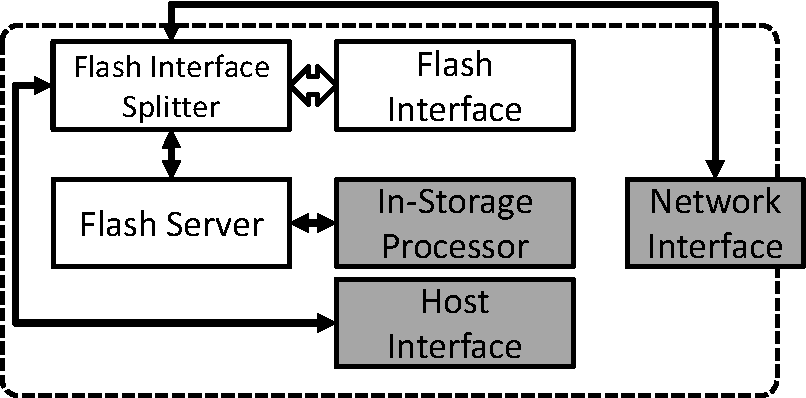
\includegraphics[scale=0.4]{figures/architecture_flash-crop.pdf}
	\caption{Flash Interface}
	\label{fig:flashinterface}
	\end{center}
\end{figure}

\subsubsection{Multiple Access Agents}

Multiple hardware endpoints in FlashBoost may need shared access to this
flash controller interface. For example, a particular controller may
be accessed by local in-store processors, local host software over PCIe
DMA, or remote in-store processors over the network. Thus we implemented a
Flash Interface Splitter with tag renaming to manage multiple users
(Figure~\ref{fig:flashinterface}). In addition, 
to ease development of hardware in-store processors,
we also provide an optional Flash Server module as part of FlashBoost. This server
converts the out-of-order and interleaved flash interface into
multiple simple in-order request/response interfaces
using page buffers. It also contains an Address Translation Unit that 
maps file handles to incoming streams of physical addresses from the host. The in-store processor
simply makes a request with the file handle, offset and length, and the Flash Server will perform
the flash operation at the corresponding physical location. The software
support for this function is discussed in Section~\ref{sec:software}). The Flash
Server's width, command queue depth and number of interfaces is adjustable 
based on the application.

\subsection{Integrated Storage Network}

\begin{figure}[h]
	\begin{center}
	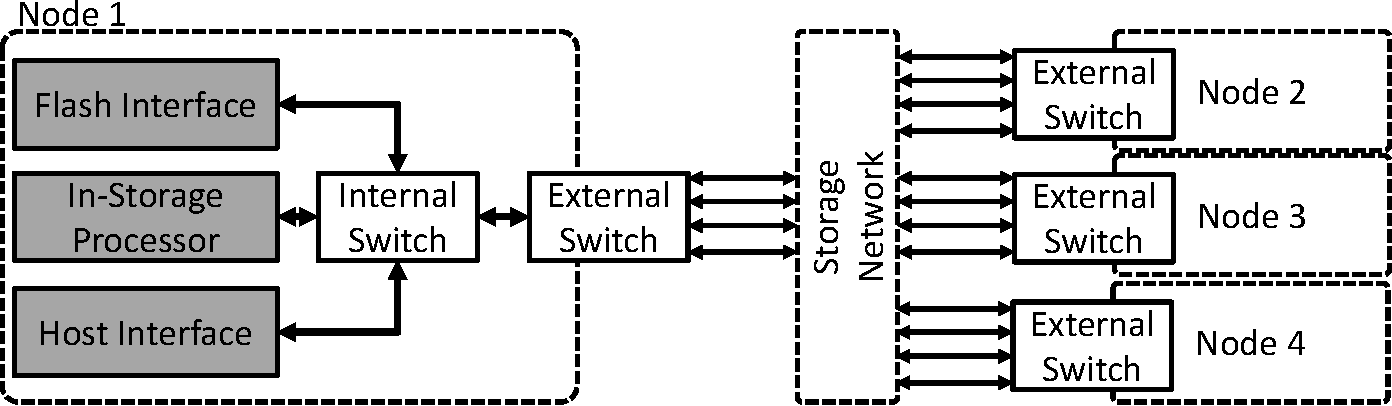
\includegraphics[width=0.5\textwidth]{figures/network-architecture-crop.pdf}
	\caption{Network Architecture}
	\label{fig:networkinterface}
	\end{center}
\end{figure}


FlashBoost provides a low-latency high-bandwidth network infrastructure across
all FlashBoost storage devices in the cluster, while maintaining a simple design
with low resource usage. FlashBoost storage devices form a separate network
among themselves via high-performance serial links.  The FlashBoost network is a
packet-switched mesh network, in which each storage device has multiple network
ports and is capable of routing packets across the network without requiring a
separate switch or router.  In addition to routing, the storage network supports functionality such as
flow control and virtual channels while maintaining high performance and
extremely low latency.  For data traffic between the storage devices, the
integrated network ports removes the overhead of going to the host software to
access a separate network interface.

Figure~\ref{fig:networkinterface} shows the network architecture. Switching is
done at two levels, the internal switch and the external switch.  The internal
switch routes packets between local components.  The external switch accesses
multiple physical network ports, and is responsible for relaying data from a
port to another port in order to relay a packet to its next hop. It is also
responsible for relaying inbound packets to the internal
switch, and relaying outbound packets from the internal switch to a correct
physical port. 

Due to the multiple ports on the storage nodes, the FlashBoost network is very
flexible and can be configured to implement various topologies, as long as no
one node requires more connections than the number of ports on it.
Figure~\ref{fig:topologies} shows some example topologies. To implement a
different topology the physical cables between each node has to be re-wired, but
the routing across a topology can be configured dynamically by the software.

%Components that want to use the network choose one or more \emph{Logical
%Endpoints}, which provide virtual channel semantics, to access the network in a
%virtualized manner.

\begin{figure}[ht!]
	\centering
	\subfloat[Distributed Star]
		{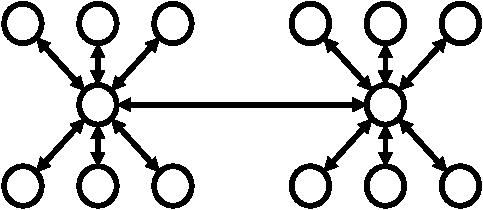
\includegraphics[scale=0.35]{figures/topology_dist_star-crop.pdf}}
		\hfill
	\subfloat[Mesh]
		{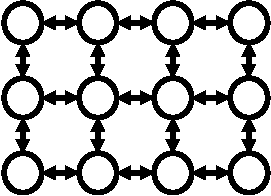
\includegraphics[scale=0.35]{figures/topology_mesh-crop.pdf}}
		\hfill
	\subfloat[Fat Tree]
		{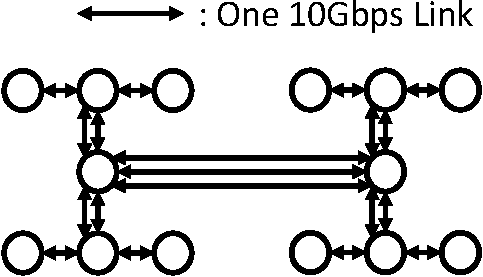
\includegraphics[scale=0.35]{figures/topology_fat_tree-crop.pdf}}
	\caption{Any Network Topology Is Possible As Long As It Requires Less Than 8
	Network Ports Per Node}
	\label{fig:topologies}
\end{figure}


\subsubsection{Logical Endpoint}

The FlashBoost network infrastructure exposes virtual channel semantics to the
users of the network by providing it with multiple \emph{logical endpoints}.  The
number of endpoints are determined at design time by setting a parameter, and
all endpoints share the physical network.  Each endpoint is parameterized with a
unique index that does not need to be contiguous.  Each endpoint exposes two
interfaces, \texttt{send} and \texttt{receive}. An in-storage processor can send
data to a remote node by calling \texttt{send} with a pair of data and
destination node index, or receive data from remote nodes by calling
\texttt{receive}, which returns a pair of data and source node index. These
interfaces provide back pressure, so that each endpoint can be treated like a
FIFO interface across the whole cluster. Such intuitive characteristics of the
network ease development of in-storage processors.

\subsubsection{Link Layer}

The link layer manages physical connections between network ports in the storage
nodes. The most important aspect of the link layer is the simple token-based
flow control implementation. This provides back pressure across the link and
assures that no packet will drop if the data rate is higher than what the
network can manage, or if the data is not received from the destination node
quick enough.

\subsubsection{Routing Layer}

%The goals of the FlashBoost network infrastructure is to
%maintain high bandwidth and low latency, while maintaining a simple design for
%embedded implementation. This requirement
%prompted many design choices.

\begin{figure}[h]
	\begin{center}
	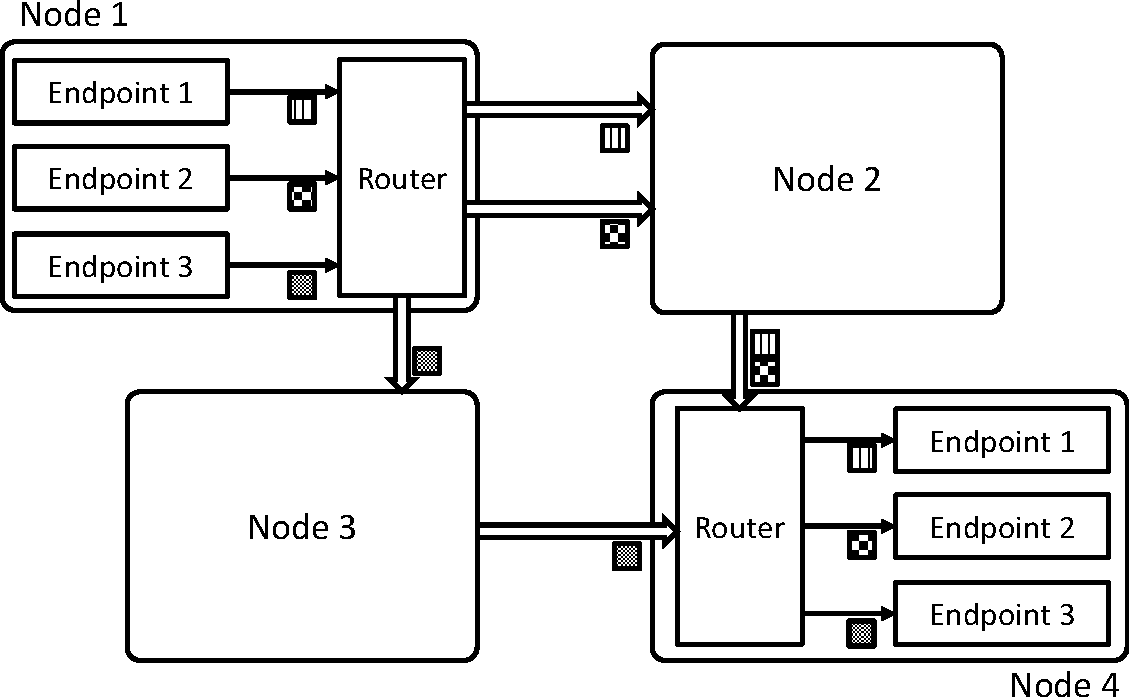
\includegraphics[width=0.4\textwidth]{figures/routing-crop.pdf}
	\caption{Routing Packets Across the Network}
	\label{fig:networkrouting}
	\end{center}
\end{figure}

In order to make maximum use of the bandwidth of the network infrastructure
while keeping resource usage to a minimal, the FlashBoost network implements
deterministic routing for each logical endpoint. This means that all packets
originating from the same logical endpoint that are directed to the same
destination node follow the same route across the network, while packets from a
different endpoint directed to the same destination node may follow a different
path. Figure~\ref{fig:networkrouting} shows packet routing in an example
network. The benefits of this approach is that packet traffic can be distributed
across multiple links, while maintaining the order of all packets from the same
endpoint. If packets from the same endpoint are allowed to take different paths,
it would require a completion buffer which may be expensive in an embedded
system.
For simplicity, the FlashBoost network does not implement a discovery protocol, and relies on a
network configuration file to populate the routing tables. 

In order to maintain extremely low network latency, each endpoint is given a
choice whether to use end-to-end flow control or not. If the developer is sure
that a particular virtual link will always drain on the receiving end, flow
end-to-end flow control can be omitted for that endpoint. However, if the
receiver fails to drain data for a long time, the link-level back pressure may
cause related parts of the network to block. On the other hand, an endpoint can
be configured to only send data when there is space on the destination endpoint,
which will assure safety but result in higher latency due to flow control
packets, and more memory usage for buffers.

\subsection{Host Interface}

The in-storage processing core can be accessed from the host server over either
a direct interface that supports RPC and DMA operations, or a file system
abstraction built on top of the direct interface. The file system interface is
described in detail in Section~\ref{sec:software}.

In order to parallelize requests and maintain high performance, the host
interface provides the software with 128 page buffers, each for reads and
writes. When writing a page, the software will request a free write buffer, copy
data to the write buffer, and send a write request over RPC with the
physical address of the destination flash page.
The buffer will be returned to the free queue when the
hardware has finished reading the data from the buffer. When reading a page, the
software will request a free read buffer, and send a read request over RPC with
the physical address of the source flash page. The software will receive an
interrupt with the buffer index when the hardware has finished writing to
software memory.

Using DMA to write data to the storage device is straightforward to parallelize,
but parallelizing reads is a bit more tricky due to the characteristics of flash
storage. When writing to storage, the DMA engine on the hardware will read data
from each buffer in order in a contiguous stream. So having enough requests in
the request queue is enough to make maximum use of the host-side link bandwidth.
However, data read from flash chips on multiple buses in parallel can arrive
interleaved at the DMA engine. Because the DMA engine needs to have enough
contiguous data for a DMA burst before issuing a DMA burst, some reordering may
be required at the DMA engine. This becomes even more tricky when the device is
using the integrated network to receive data from remote nodes, where they might
all be coming from different buses. To fix this issue, we provide dual-ported
buffer in hardware providing the semantics of a vector of FIFOs, so that data
for each request can be enqueued into its own FIFO until there is enough data
for a burst.
Figure~\ref{fig:hostinterface} describes the structure of the host interface for
flash reads.

\begin{figure}[ht!]
	\centering
	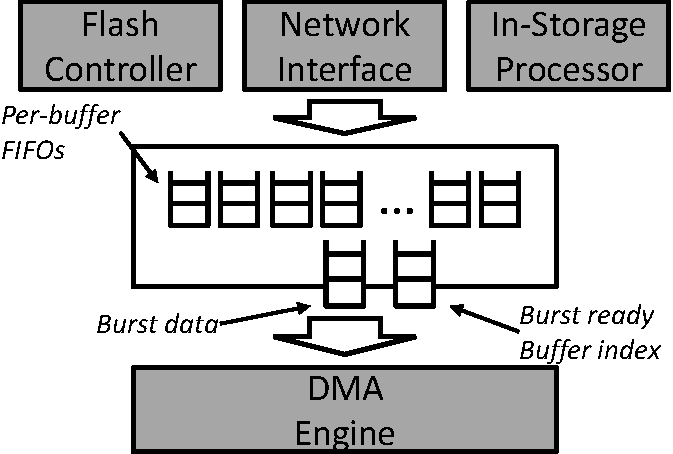
\includegraphics[width=0.3\textwidth]{figures/dmawrite-crop.pdf}
	\caption{Host-FPGA Interface Over PCIe}
	\label{fig:hostinterface}
\end{figure}

%TODO: \subsubsection{Storage Bridge to Host}


%%%% Comments!

\begin{comment}
The raw flash interface, in hardware, is defined below:

%[captionpos=b, caption={Flash Controller Interface}, label={lst:hwifc}]
\begin{lstlisting}
interface FlashIfc;       
  method sendCmd (FlashOp op, Bit#(4) bus,
                  Bit#(3) chip, Bit#(16) block, 
                  Bit#(8) page, Bit#(8) tag);        
  method writeWord (Bit#(128) data, Bit#(8) tag);
  method Tuple2#(Bit#(128), Bit#(8)) readWord (); 
  method Bit#(8) writeDataReq ();
  method Tuple2#(Bit#(8), StatusT) ackStatus ();
endinterface 
\end{lstlisting}
\end{comment}

